% =====================================================================
\chapter{Integrales dobles y la integral gaussiana}
\label{tema:6}
% =====================================================================

La integral de una variable suma los valores de una función a lo largo de un intervalo; la integral doble los suma sobre una región del plano y mide, por ejemplo, el volumen bajo una superficie. Su cálculo se reduce a dos integrales de una variable sucesivas (teorema de Fubini), y en regiones circulares conviene usar coordenadas polares. La aplicación más importante para el curso es el cálculo de la integral gaussiana $\int_{-\infty}^{\infty}e^{-x^2}dx=\sqrt\pi$, que no puede obtenerse con primitivas elementales y sí con un rodeo por el plano. La presentación sigue las sesiones~47--54 de 18.02SC~\cite{mit1802}, las §5.1--5.3 de OpenStax~\cite{openstax3}, las §11.1--11.14 de Apostol~\cite{apostol2} y las §14.1--14.2 de Strang~\cite{strangcalc}.

\section{Integral doble sobre un rectángulo}

Sea $R=[a,b]\times[c,d]$ y $f$ acotada en $R$. Se divide $[a,b]$ en $m$ subintervalos de longitud $\Delta x$ y $[c,d]$ en $n$ de longitud $\Delta y$, lo que divide $R$ en $mn$ rectángulos $R_{ij}$ de área $\Delta A=\Delta x\,\Delta y$, y se elige un punto $(x_{ij}^*,y_{ij}^*)$ en cada uno.

\begin{definicion}[Integral doble]\label{def:integral-doble}
La \emph{integral doble} de $f$ sobre $R$ es
\[
\iint_R f(x,y)\dA=\lim_{m,n\to\infty}\sum_{i=1}^{m}\sum_{j=1}^{n}f(x_{ij}^*,y_{ij}^*)\,\Delta A ,
\]
si el límite existe y no depende de la elección de los puntos; se dice entonces que $f$ es \emph{integrable} en $R$. Toda función continua en $R$ es integrable.
\end{definicion}

Si $f\ge0$, cada sumando es el volumen de un prisma de base $R_{ij}$ y altura $f(x_{ij}^*,y_{ij}^*)$, y la integral es el \emph{volumen} del sólido comprendido entre $R$ y la gráfica de $f$. Si $f=1$, la integral es el área de $R$.

\begin{proposicion}[Propiedades]\label{prop:propiedades-integral}
Para $f,g$ integrables en $R$ y $\alpha,\beta\in\R$:
\begin{enumerate}
  \item linealidad: $\iint_R(\alpha f+\beta g)\dA=\alpha\iint_Rf\dA+\beta\iint_Rg\dA$;
  \item monotonía: si $f\le g$ en $R$, entonces $\iint_Rf\dA\le\iint_Rg\dA$;
  \item aditividad: si $R$ se divide en dos regiones $R_1$, $R_2$ que solo comparten frontera, $\iint_R f=\iint_{R_1}f+\iint_{R_2}f$.
\end{enumerate}
\end{proposicion}

Las tres propiedades se heredan de las sumas de Riemann al pasar al límite: por ejemplo, si $f\le g$, cada suma de $f$ es menor o igual que la correspondiente de $g$. El cálculo efectivo se apoya en el teorema siguiente, cuya demostración puede verse en Apostol~\cite[§11.10--11.11]{apostol2}.

\begin{teorema}[Fubini, para rectángulos]\label{teo:fubini}
Si $f$ es continua en $R=[a,b]\times[c,d]$, entonces
\[
\iint_R f\dA=\int_a^b\left(\int_c^d f(x,y)\,dy\right)dx=\int_c^d\left(\int_a^b f(x,y)\,dx\right)dy .
\]
\end{teorema}

En la integral interior $\int_c^df(x,y)\,dy$, la variable $x$ se trata como constante. Geométricamente, es el área de la sección del sólido por el plano vertical de abscisa $x$, y el volumen se obtiene sumando secciones.

\begin{corolario}[Integrandos separables]\label{cor:separable}
Si $f(x,y)=g(x)h(y)$ con $g$ y $h$ continuas, entonces $\iint_{[a,b]\times[c,d]}g(x)h(y)\dA=\left(\int_a^bg\right)\left(\int_c^dh\right)$.
\end{corolario}

\begin{proof}
Por Fubini, la integral es $\int_a^b\bigl(\int_c^dg(x)h(y)\,dy\bigr)dx$. En la integral interior $g(x)$ es constante: $\int_c^dg(x)h(y)\,dy=g(x)\int_c^dh$. Sacando la constante $\int_c^dh$ de la integral exterior se obtiene el resultado.
\end{proof}

\begin{ejemplo}\label{ej:t6-rectangulo}
$\iint_{[0,2]\times[0,3]}xy^2\dA=\int_0^2x\,dx\cdot\int_0^3y^2\,dy=2\cdot9=18$. Con Fubini sin separar: $\int_0^2\bigl[\tfrac{xy^3}{3}\bigr]_{y=0}^{y=3}dx=\int_0^29x\,dx=18$.
\end{ejemplo}

\section{Regiones generales y cambio del orden de integración}

\begin{definicion}[Regiones elementales]\label{def:regiones}
Una región es \emph{de tipo~I} si es de la forma $\{a\le x\le b,\ g_1(x)\le y\le g_2(x)\}$, y \emph{de tipo~II} si es $\{c\le y\le d,\ h_1(y)\le x\le h_2(y)\}$, con $g_i$, $h_i$ continuas.
\end{definicion}

Para $f$ continua, el teorema de Fubini se extiende a estas regiones~\cite[§11.12--11.14]{apostol2}:
\begin{align*}
\iint_Df\dA&=\int_a^b\int_{g_1(x)}^{g_2(x)}f(x,y)\,dy\,dx&&\text{(tipo I)},\\
\iint_Df\dA&=\int_c^d\int_{h_1(y)}^{h_2(y)}f(x,y)\,dx\,dy&&\text{(tipo II)}.
\end{align*}
Los límites de la integral interior pueden depender de la variable exterior; los de la exterior han de ser constantes. El método práctico es: dibujar la región, fijar la variable exterior y leer, sobre un segmento vertical (tipo~I) u horizontal (tipo~II), dónde entra y dónde sale de la región.

\begin{ejemplo}\label{ej:t6-region}
Sea $D$ la región entre $y=x^2$ e $y=x$ para $0\le x\le1$ (las curvas se cortan en $x=0$ y $x=1$, y $x^2\le x$ en medio). Entonces
\[
\iint_D(x+y)\dA=\int_0^1\int_{x^2}^{x}(x+y)\,dy\,dx=\int_0^1\Bigl(\tfrac32x^2-x^3-\tfrac12x^4\Bigr)dx=\tfrac12-\tfrac14-\tfrac1{10}=\tfrac{3}{20}.
\]
\end{ejemplo}

Cuando la integral interior no tiene primitiva elemental, puede bastar con cambiar el orden. Hay que describir la \emph{misma} región del otro modo.

\begin{ejemplo}\label{ej:t6-orden}
La integral $\int_0^1\int_x^1\sin(y^2)\,dy\,dx$ no puede calcularse en ese orden. La región es el triángulo $\{0\le x\le1,\ x\le y\le1\}$, que como región de tipo~II es $\{0\le y\le1,\ 0\le x\le y\}$. Por tanto,
\[
\int_0^1\int_0^y\sin(y^2)\,dx\,dy=\int_0^1y\sin(y^2)\,dy=\Bigl[-\tfrac12\cos(y^2)\Bigr]_0^1=\frac{1-\cos1}{2}\approx0{,}2298 .
\]
\end{ejemplo}

\section{Coordenadas polares}

En polares, $x=r\cos\theta$, $y=r\sin\theta$, con $r\ge0$. Las regiones naturales son los \emph{rectángulos polares} $\{r_1\le r\le r_2,\ \theta_1\le\theta\le\theta_2\}$, sectores de corona circular. Su área es la diferencia de dos sectores circulares:
\[
\tfrac12r_2^2\Delta\theta-\tfrac12r_1^2\Delta\theta=\tfrac{r_1+r_2}{2}\,(r_2-r_1)\,\Delta\theta=\bar r\,\Delta r\,\Delta\theta ,
\]
donde $\bar r$ es el radio medio. Así, un rectángulo polar pequeño tiene área aproximada $r\,\Delta r\,\Delta\theta$, no $\Delta r\,\Delta\theta$: los rectángulos más alejados del origen son más grandes. Sumando y pasando al límite se obtiene el resultado siguiente~\cite[§11.26--11.31]{apostol2}.

\begin{teorema}[Cambio a coordenadas polares]\label{teo:polares}
Si $f$ es continua en la región $D=\{\alpha\le\theta\le\beta,\ r_1(\theta)\le r\le r_2(\theta)\}$, con $0\le\beta-\alpha\le2\pi$, entonces
\[
\iint_Df(x,y)\dA=\int_\alpha^\beta\int_{r_1(\theta)}^{r_2(\theta)}f(r\cos\theta,r\sin\theta)\,r\,dr\,d\theta .
\]
\end{teorema}

El factor $r$ es el valor absoluto del determinante de las derivadas parciales de $(x,y)$ respecto de $(r,\theta)$, el \emph{jacobiano} $\bigl|\begin{smallmatrix}\cos\theta&-r\sin\theta\\\sin\theta&r\cos\theta\end{smallmatrix}\bigr|=r$, de acuerdo con la interpretación del determinante como factor de cambio de área (\cref{teo:det-area}).

\begin{ejemplo}\label{ej:t6-polares}
El volumen bajo el paraboloide $z=1-x^2-y^2$ y sobre el disco unidad es
\[
\int_0^{2\pi}\int_0^1(1-r^2)\,r\,dr\,d\theta=2\pi\Bigl[\tfrac{r^2}{2}-\tfrac{r^4}{4}\Bigr]_0^1=2\pi\cdot\tfrac14=\frac\pi2 .
\]
\end{ejemplo}

\section{La integral gaussiana}

\begin{teorema}[Integral gaussiana]\label{teo:gauss}
La integral impropia $\int_{-\infty}^{\infty}e^{-x^2}dx$ converge y vale $\sqrt\pi$.
\end{teorema}

\begin{proof}
\emph{Convergencia.} Para $\abs x\ge1$ se tiene $x^2\ge\abs x$, luego $0<e^{-x^2}\le e^{-\abs x}$, cuya integral sobre $\abs x\ge1$ es finita; por comparación, la integral converge. Sea $I(R)=\int_{-R}^{R}e^{-x^2}dx$, que tiende al valor buscado cuando $R\to\infty$.

\emph{Paso al plano.} Por el \cref{cor:separable}, con $S_R=[-R,R]^2$,
\[
I(R)^2=\int_{-R}^{R}e^{-x^2}dx\int_{-R}^{R}e^{-y^2}dy=\iint_{S_R}e^{-(x^2+y^2)}\dA .
\]
\emph{Comparación con discos.} Sea $D_\rho$ el disco de centro el origen y radio $\rho$. Se tiene $D_R\subseteq S_R\subseteq D_{R\sqrt2}$ (\cref{fig:t6-gauss}), y como el integrando es positivo, la aditividad y la monotonía dan
\[
\iint_{D_R}e^{-(x^2+y^2)}\dA\le I(R)^2\le\iint_{D_{R\sqrt2}}e^{-(x^2+y^2)}\dA .
\]
\emph{Cálculo en polares.} Por el \cref{teo:polares},
\[
\iint_{D_\rho}e^{-(x^2+y^2)}\dA=\int_0^{2\pi}\int_0^{\rho}e^{-r^2}r\,dr\,d\theta=2\pi\Bigl[-\tfrac12e^{-r^2}\Bigr]_0^{\rho}=\pi\bigl(1-e^{-\rho^2}\bigr).
\]
Por tanto, $\pi(1-e^{-R^2})\le I(R)^2\le\pi(1-e^{-2R^2})$. Ambas cotas tienden a $\pi$ cuando $R\to\infty$; por el principio del sándwich, $I(R)^2\to\pi$ y, como $I(R)>0$, $I(R)\to\sqrt\pi$.
\end{proof}

\begin{figure}[ht]
\centering
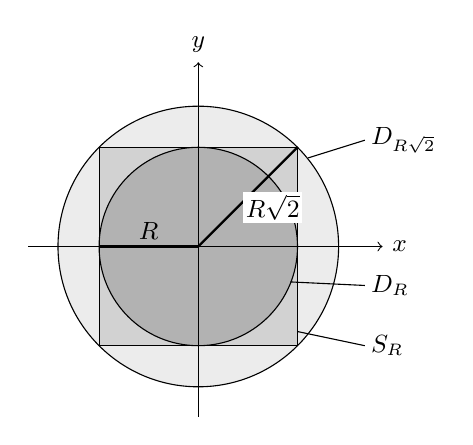
\begin{tikzpicture}[scale=0.9,font=\small]
  \fill[gray!15] (0,0) circle ({1.4*sqrt(2)});
  \fill[gray!35] (-1.4,-1.4) rectangle (1.4,1.4);
  \fill[gray!60] (0,0) circle (1.4);
  \draw (0,0) circle ({1.4*sqrt(2)}); \draw (-1.4,-1.4) rectangle (1.4,1.4); \draw (0,0) circle (1.4);
  \draw[->] (-2.4,0) -- (2.6,0) node[right] {$x$};
  \draw[->] (0,-2.4) -- (0,2.6) node[above] {$y$};
  \draw[thick] (0,0) -- (1.4,1.4);
  \node[fill=white,inner sep=1pt] at (1.05,0.55) {$R\sqrt2$};
  \draw[thick] (0,0) -- (-1.4,0);
  \node[above,fill=gray!60,inner sep=1pt] at (-0.7,0.05) {$R$};
  \node[right] at (2.3,1.5) {$D_{R\sqrt2}$}; \draw (2.35,1.5) -- (1.55,1.25);
  \node[right] at (2.3,-1.4) {$S_R$}; \draw (2.35,-1.4) -- (1.4,-1.2);
  \node[right] at (2.3,-0.55) {$D_R$}; \draw (2.35,-0.55) -- (1.3,-0.5);
\end{tikzpicture}
\caption{El cuadrado $S_R$ contiene al disco $D_R$ y está contenido en $D_{R\sqrt2}$. Las integrales de $e^{-(x^2+y^2)}$ sobre los discos se calculan en polares y encierran a $I(R)^2$.}
\label{fig:t6-gauss}
\end{figure}

\begin{corolario}\label{cor:gauss-normal}
$\displaystyle\int_{-\infty}^{\infty}e^{-x^2/2}\,dx=\sqrt{2\pi}$. En consecuencia, la densidad normal estándar $\varphi(x)=\frac{1}{\sqrt{2\pi}}e^{-x^2/2}$ integra~$1$.
\end{corolario}

\begin{proof}
Con el cambio $x=\sqrt2\,u$, $dx=\sqrt2\,du$: $\int e^{-x^2/2}dx=\sqrt2\int e^{-u^2}du=\sqrt2\sqrt\pi$.
\end{proof}

\begin{observacion}[Errores frecuentes]
\begin{enumerate}[label=(\alph*)]
\item Olvidar el factor $r$ en $dA=r\,dr\,d\theta$. Sin él, el área del disco unidad saldría $2\pi$ en lugar de $\pi$.
\item Poner en la integral exterior límites que dependen de la otra variable: el resultado de una integral doble es un número.
\item Cambiar el orden de integración intercambiando sin más los límites. Hay que redibujar la región y describirla de nuevo (\cref{ej:t6-orden}).
\item Aplicar el \cref{cor:separable} cuando la región no es un rectángulo: sobre un triángulo, $\iint g(x)h(y)\dA$ no es en general el producto de dos integrales.
\end{enumerate}
\end{observacion}

\begin{observacion}[Conexión con el curso]
La distribución normal, omnipresente en el curso (inicialización de los pesos, ruido, teorema central del límite), se define con la densidad del \cref{cor:gauss-normal}; su normalización y el cálculo de su varianza se apoyan en este tema (módulo~5, tema~3, y \cref{eje:6-gaussiana-normal}). Las integrales dobles aparecen también en la entropía diferencial de una normal (módulo~6) y en el cálculo de probabilidades conjuntas de dos variables continuas (módulo~5).
\end{observacion}

\begin{lecturas}
\item MIT 18.02SC~\cite{mit1802}, unidad~3, parte~A, sesiones~47--50 (definición, ejemplos, cambio de orden, polares) y~51 (masa y valor medio).
\item OpenStax \emph{Calculus}, vol.~3~\cite{openstax3}, §5.1 «Double Integrals over Rectangular Regions», §5.2 «Double Integrals over General Regions» y §5.3 «Double Integrals in Polar Coordinates».
\item Apostol~\cite{apostol2}, §11.1--11.14 (integral doble, Fubini, regiones generales) y §11.26--11.31 (cambio de variables).
\item Strang, \emph{Calculus}~\cite{strangcalc}, §14.1 «Double Integrals» y §14.2 «Changing to Better Coordinates».
\end{lecturas}

\section*{Ejercicios del tema 6}
\addcontentsline{toc}{section}{Ejercicios del tema 6}

\begin{ejercicio}{1}{eje:6-simetria}
Sea $D$ el disco unidad centrado en el origen. Sin calcular, decida cuáles de las integrales siguientes son nulas por simetría y, para las demás, escriba una integral equivalente sobre un semidisco o un cuarto de disco: $\iint_Dx\dA$, $\iint_De^x\dA$, $\iint_Dx^2\dA$, $\iint_Dx^2y\dA$, $\iint_D(x^2+y)\dA$, $\iint_Dxy\dA$.
\fuente{adaptado de MIT 18.02SC~\cite{mit1802}, problemas suplementarios, 3A-6.}
\end{ejercicio}

\begin{ejercicio}{2}{eje:6-iteradas}
Calcule: (a) $\displaystyle\int_0^2\int_{-1}^{1}(6x^2+2y)\,dy\,dx$; (b) $\displaystyle\int_0^1\int_0^{u}\sqrt{u^2+4}\,dv\,du$.
\fuente{adaptado de MIT 18.02SC~\cite{mit1802}, problemas suplementarios, 3A-1.}
\end{ejercicio}

\begin{ejercicio}{2}{eje:6-rectangulos}
Calcule sobre los rectángulos indicados: (a) $\iint(x+y)^2\dA$ en $[0,1]\times[0,2]$; (b) $\iint\sin(x+y)\dA$ en $[0,\frac\pi2]\times[0,\frac\pi2]$; (c) $\iint xe^{xy}\dA$ en $[0,1]\times[0,1]$, eligiendo el orden más cómodo.
\fuente{adaptado de OpenStax \emph{Calculus}, vol.~3~\cite{openstax3}, §5.1.}
\end{ejercicio}

\begin{ejercicio}{2}{eje:6-planteo}
Escriba $\iint_Df\dA$ como integral iterada en los dos órdenes, $dy\,dx$ y $dx\,dy$: (a) $D$ es el triángulo de vértices $(0,0)$, $(0,2)$ y $(-2,2)$; (b) $D$ es la región finita comprendida entre la parábola $y=2x-x^2$ y el eje $x$. Calcule el área de la región (b).
\fuente{adaptado de MIT 18.02SC~\cite{mit1802}, problemas suplementarios, 3A-2.}
\end{ejercicio}

\begin{ejercicio}{2}{eje:6-region}
Calcule $\iint_Dx\dA$, donde $D$ es la región limitada por los ejes coordenados y la recta $2y+x=2$.
\fuente{adaptado de MIT 18.02SC~\cite{mit1802}, problemas suplementarios, 3A-3.}
\end{ejercicio}

\begin{ejercicio}{2}{eje:6-volumen-xy}
Halle el volumen del sólido situado bajo la superficie $z=xy$ y sobre la región del primer cuadrante comprendida entre las curvas $y=x$ e $y=x^2$.
\fuente{adaptado de MIT 18.02SC~\cite{mit1802}, problemas suplementarios, 3A-4.}
\end{ejercicio}

\begin{ejercicio}{2}{eje:6-orden-1}
Calcule $\displaystyle\int_0^2\int_x^2e^{-y^2}\,dy\,dx$ cambiando el orden de integración.
\fuente{adaptado de MIT 18.02SC~\cite{mit1802}, problemas suplementarios, 3A-5.}
\end{ejercicio}

\begin{ejercicio}{2}{eje:6-orden-2}
Calcule $\displaystyle\int_0^1\int_{\sqrt[3]{x}}^{1}\frac{1}{1+u^4}\,du\,dx$ cambiando el orden de integración.
\fuente{adaptado de MIT 18.02SC~\cite{mit1802}, problemas suplementarios, 3A-5.}
\end{ejercicio}

\begin{ejercicio}{2}{eje:6-polares}
Calcule, pasando a polares, $\displaystyle\iint_D\frac{dx\,dy}{1+x^2+y^2}$, donde $D$ es la parte del disco $x^2+y^2\le a^2$ situada en el primer cuadrante.
\fuente{adaptado de MIT 18.02SC~\cite{mit1802}, problemas suplementarios, 3B-2.}
\end{ejercicio}

\begin{ejercicio}{2}{eje:6-semiesfera}
Calcule en polares el volumen de una semiesfera maciza de radio $a$, es decir, el volumen bajo $z=\sqrt{a^2-x^2-y^2}$ sobre el disco $x^2+y^2\le a^2$.
\fuente{adaptado de MIT 18.02SC~\cite{mit1802}, problemas suplementarios, 3B-3.}
\end{ejercicio}

\begin{ejercicio}{2}{eje:6-centroide}
El \emph{centroide} de una región $D$ es el punto $(\bar x,\bar y)$ con $\bar x=\frac{1}{\text{área}(D)}\iint_Dx\dA$ e $\bar y$ análogo. Halle el centroide del sector circular de radio $a$ y ángulo central $2\alpha$ ($0<\alpha\le\pi$) colocado simétricamente respecto del eje $x$, con el vértice en el origen. Particularice al semidisco.
\fuente{adaptado de MIT 18.02SC~\cite{mit1802}, problemas suplementarios, 3C-4.}
\end{ejercicio}

\begin{ejercicio}{2}{eje:6-gauss-polar}
(a) Calcule $\iint_{x^2+y^2\le R^2}e^{-(x^2+y^2)}\dA$. (b) ¿Para qué radio $R$ es esa integral el 99\,\% de su valor sobre todo el plano?
\end{ejercicio}

\begin{ejercicio}{3}{eje:6-capas}
Sea $z=f(r)\ge0$ una superficie de revolución alrededor del eje $z$, con $f$ continua en $[0,a]$. (a) Demuestre que la fórmula en polares del volumen bajo la superficie y sobre el disco $r\le a$ coincide con la fórmula de las capas cilíndricas del cálculo de una variable, $V=\int_0^a2\pi r f(r)\,dr$. (b) Aplíquela al cono $f(r)=h(1-r/a)$ y compruebe que se obtiene $\frac13\pi a^2h$.
\fuente{adaptado de MIT 18.02SC~\cite{mit1802}, \emph{problem set}~7, parte~II, problema~2.}
\end{ejercicio}

\begin{ejercicio}{3}{eje:6-cota}
Demuestre, sin calcular la integral, que $\displaystyle\iint_{[0,1]^2}\frac{x}{1+x^2+y^2}\dA<0{,}35$. (Indicación: acote el integrando por una función de $x$ sola y use la monotonía.)
\fuente{adaptado de MIT 18.02SC~\cite{mit1802}, problemas suplementarios, 3A-7.}
\end{ejercicio}

\begin{ejercicio}{3}{eje:6-gaussiana-normal}
(a) Demuestre que $\int_{-\infty}^{\infty}e^{-(x-\mu)^2/(2\sigma^2)}dx=\sigma\sqrt{2\pi}$ para $\mu\in\R$ y $\sigma>0$. (b) Demuestre, integrando por partes, que $\int_{-\infty}^{\infty}x^2e^{-x^2/2}dx=\sqrt{2\pi}$. (c) Deduzca que si $X$ tiene densidad $\varphi(x)=\frac1{\sqrt{2\pi}}e^{-x^2/2}$, entonces $\E[X]=0$ y $\E[X^2]=1$.
\end{ejercicio}
